\documentclass{standalone}

\begin{document}

\appendix

\section{Plots}

Features' Correlation within each category, i.e., \lstinline{ind}, \lstinline{reg}, \lstinline{car}, \lstinline{calc} are shown as histograms in \cref{corr_ind}, \cref{corr_reg}, \cref{corr_car} and \cref{corr_calc} respectfully.

\begin{figure}[!bt]
\centering
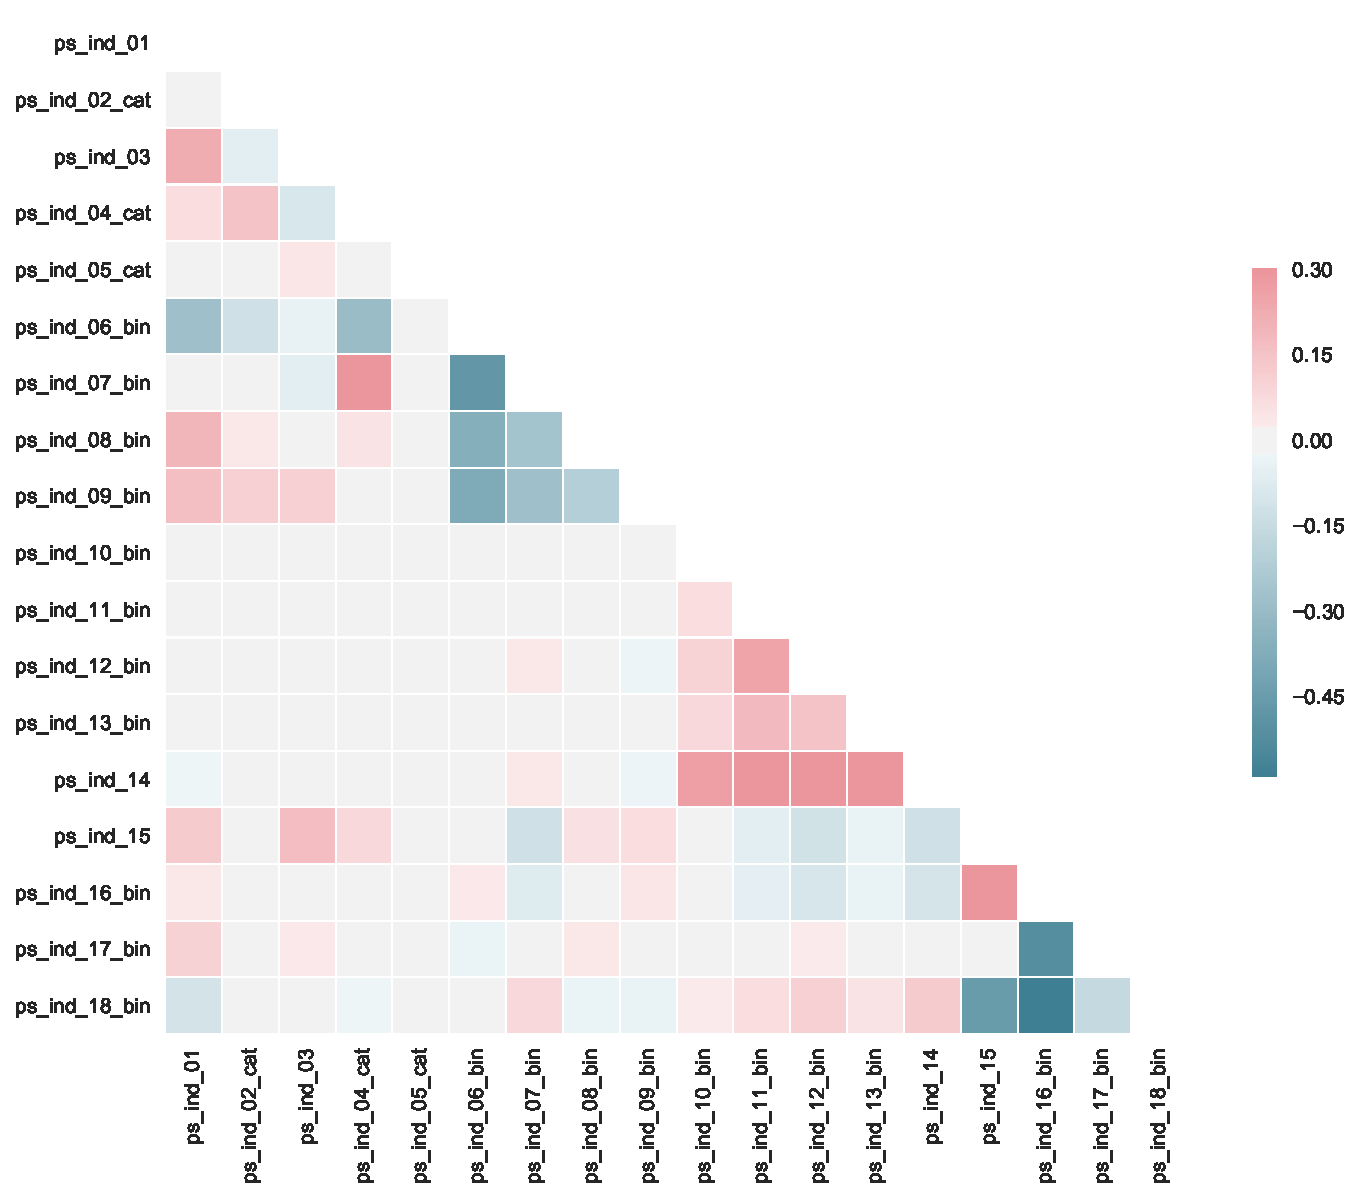
\includegraphics[width=.5\textwidth]{fig/corr_ind_col.pdf}
\caption{Correlation for the \lstinline{ind} Attributes.}
\label{corr_ind}
\end{figure}

\begin{figure}[!bt]
\centering
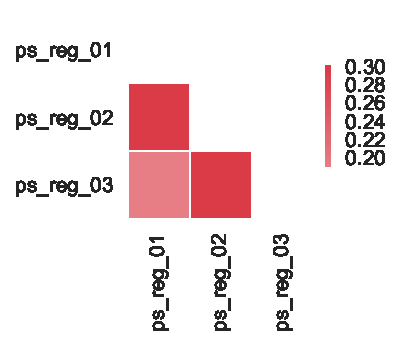
\includegraphics[width=.2\textwidth]{fig/corr_reg_col.pdf}
\caption{Histogram for the \lstinline{reg} Attributes.}
\label{corr_reg}
\end{figure}

\begin{figure}[!bt]
\centering
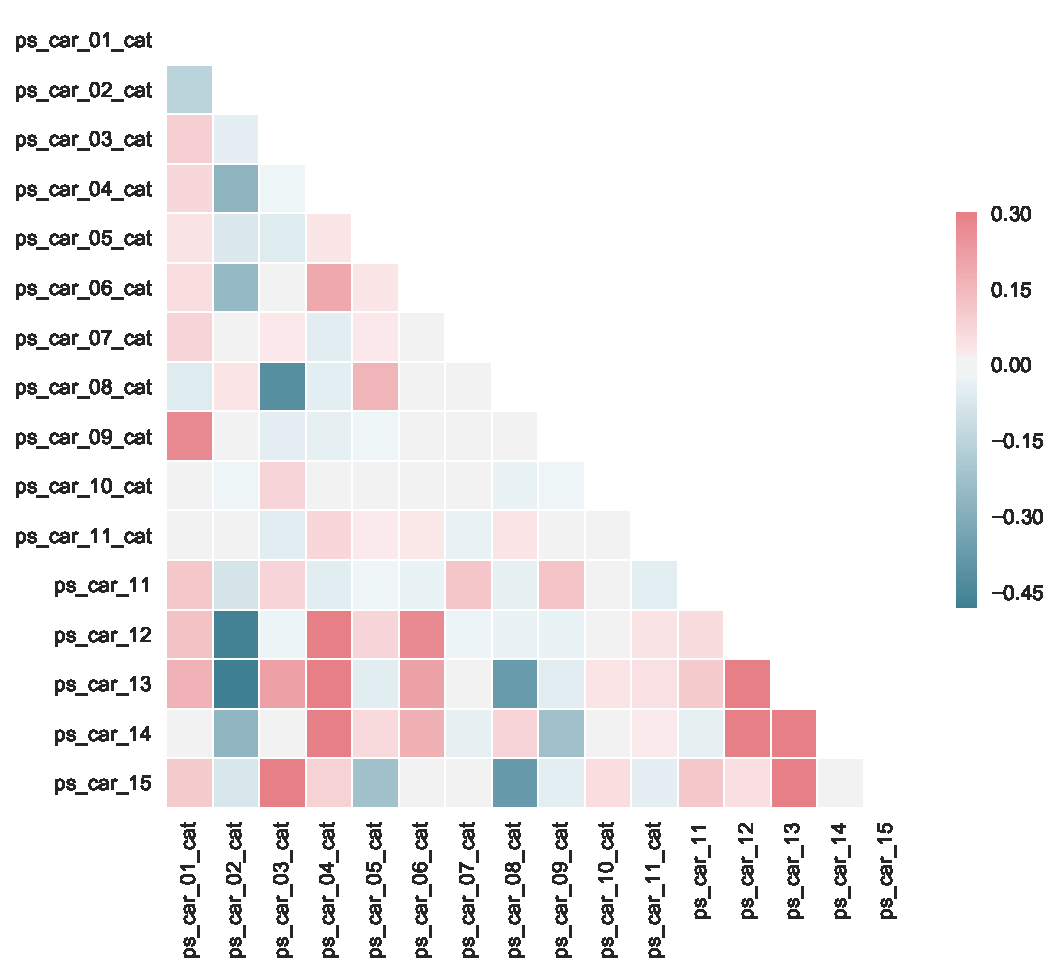
\includegraphics[width=.5\textwidth]{fig/corr_car_col.pdf}
\caption{Histogram for the \lstinline{car} Attributes.}
\label{corr_car}
\end{figure}

\begin{figure}[!bt]
\centering
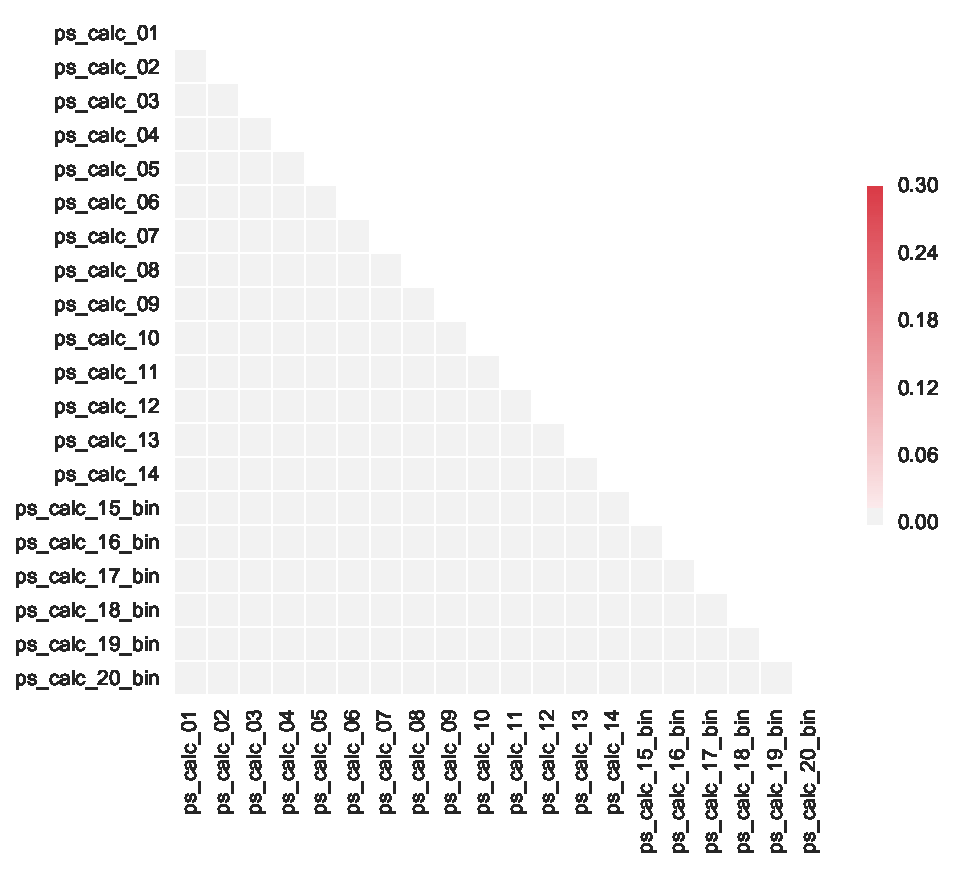
\includegraphics[width=.5\textwidth]{fig/corr_calc_col.pdf}
\caption{Histogram for the \lstinline{calc} Attributes.}
\label{corr_calc}
\end{figure}

\end{document}